\chapter{Imperative Paradigm}
\label{ch:p1}

\section{Problem Statement}
\label{sec:pm1}

Compute distance between two documents.

\section{Data Structures and algorithms}

Some basic data structures like lists and dictionaries were used. Term frequency–inverse document frequency (Tf-Idf), is a numerical statistic that is intended to reflect how important a word is to a document in a collection or corpus. This method has been used to give weightage to more important words rather than just the word frequency.

\section{Design decisions}

Tf-idf weights are used to give weights to various words. Even though Tf-Idf reduces the weight to commonly used words, we opted to remove such words from word frequency vector to remove even minor weightage given to such words.\\
\indent This way weight of other important words increases. While parsing the text, we decided not to use \$ and \% as delimiters as they could have some importance as \$ could mean money and \% could imply percentage 


\section{Methodology}

The entire methodology is divide into 4 stages. These include formatting text, creating word frequency vector, computing tf-idf weights and calculation of distance. 

\begin{figure}[H]
	\centering
	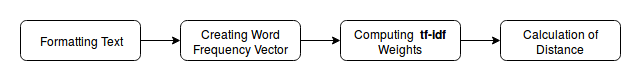
\includegraphics[height=0.12\textwidth,keepaspectratio]{flow_chart.png}\\
	\caption{The flow chart depicting stages of algorithm}
\end{figure}

\begin{itemize}
	\item \textbf{Formatting text :} Read the file and extract words from it. Words are obtained by splitting the text by various delimiters (variable \verb|delimiters|).
	\item \textbf{Word frequency vector :} After extracting the words, a vector that contains the frequency of each and every word is created. The vector is saved in a dictionary. This is done for each and every file in the corpus.
	\item \textbf{Computing tf-idf weights :} Tf-Idf weights corresponding to the above word frequency vector is calculated as per the given formula.
	\begin{center}
		$TF(t) = \frac{\text{Number of times term t appears in a document}}{\text{Total number of terms in the document}}$\\ 
		\vspace{1.2em}
		$IDF(t) = \ln \big( {\frac{\text{Total number of documents}}{\text{ Number of documents with term t in it}}} \big) $\\
		\vspace{1.2em}
		Tf-idf weight(t) = TF(t) * IDF(t)
	\end{center}
	\item \textbf{Calculation of distance :} The distance between each and every pair of files is done by calculating the cosine distance and saved in a list. This list is sorted in ascending order and logged to a file. 
\end{itemize}

\section{Observations and results}
\label{sec:p01}

Some interesting observations have been found. Distance between same files is zero. The time taken for calculating the result for 1000 documents, total size (of all files) 2.6 MB is approximately 1100 seconds.

\section{Contribution of team members}

All the  members of the team have put their maximum efforts. Every one helped each other throughout the project, both in debugging of the code as well conceptual part. All the members have put the same amount of man hours for this project. So, one cannot pinpoint of less contribution of any particular member of the team.\\
\indent Every one has helped in writing the each and every part of code and also in writing of report. However, if one needs to exactly know the division of labour. This is as follows:\\


\begin{center}
	\begin{tabular}{ c c  }
		\textbf{Jayaprakash A} &  Tf-Idf vectorisation  \\ 
		\textbf{Siddhardha SST} & Creating word frequency vector\\  
		\textbf{Mettu Aditya} &  Text retrieval and mining\\
		 \textbf{Vinay Ande} &   Calculation of cosine distance\\
	\end{tabular}
\end{center}


